
\documentclass[8pt]{article}

\usepackage[utf8]{inputenc}

\usepackage{amsmath, bm}
\usepackage{graphicx}
\usepackage{amssymb}
\usepackage{float}
\usepackage{caption}
\usepackage{subcaption}
% set font size to 11pt
% set margin
\usepackage[margin=0.5in]{geometry}


\begin{document}

% insert pdf cover page here

\title{Lab report: 3A3 Supersonic Nozzle}
\author{lwp26}
\date{October 2023}
\maketitle

\section{Part 1 Convergent - divergent nozzle}

In this short report, the flow through a convergent - divergent nozzle is analysed in four cases.

\begin{itemize}
    \item Case 1: Subsonic flow throughout the nozzle
    \item Case 2: Choked flow at the throat then subsonic exit flow
    \item Case 3: Choked flow at the throat, then supersonic exit flow with a shock wave in the nozzle divergence
    \item Case 4: Choked flow at the throat, then supersonic exit flow
\end{itemize}

The downstream static pressue is controlled by a valve to set the operating point of the nozzle.

Nozzle layout for part 1 experiment shown in figure \ref{fig:figure1} below.

\begin{figure}[H]
    \centering
    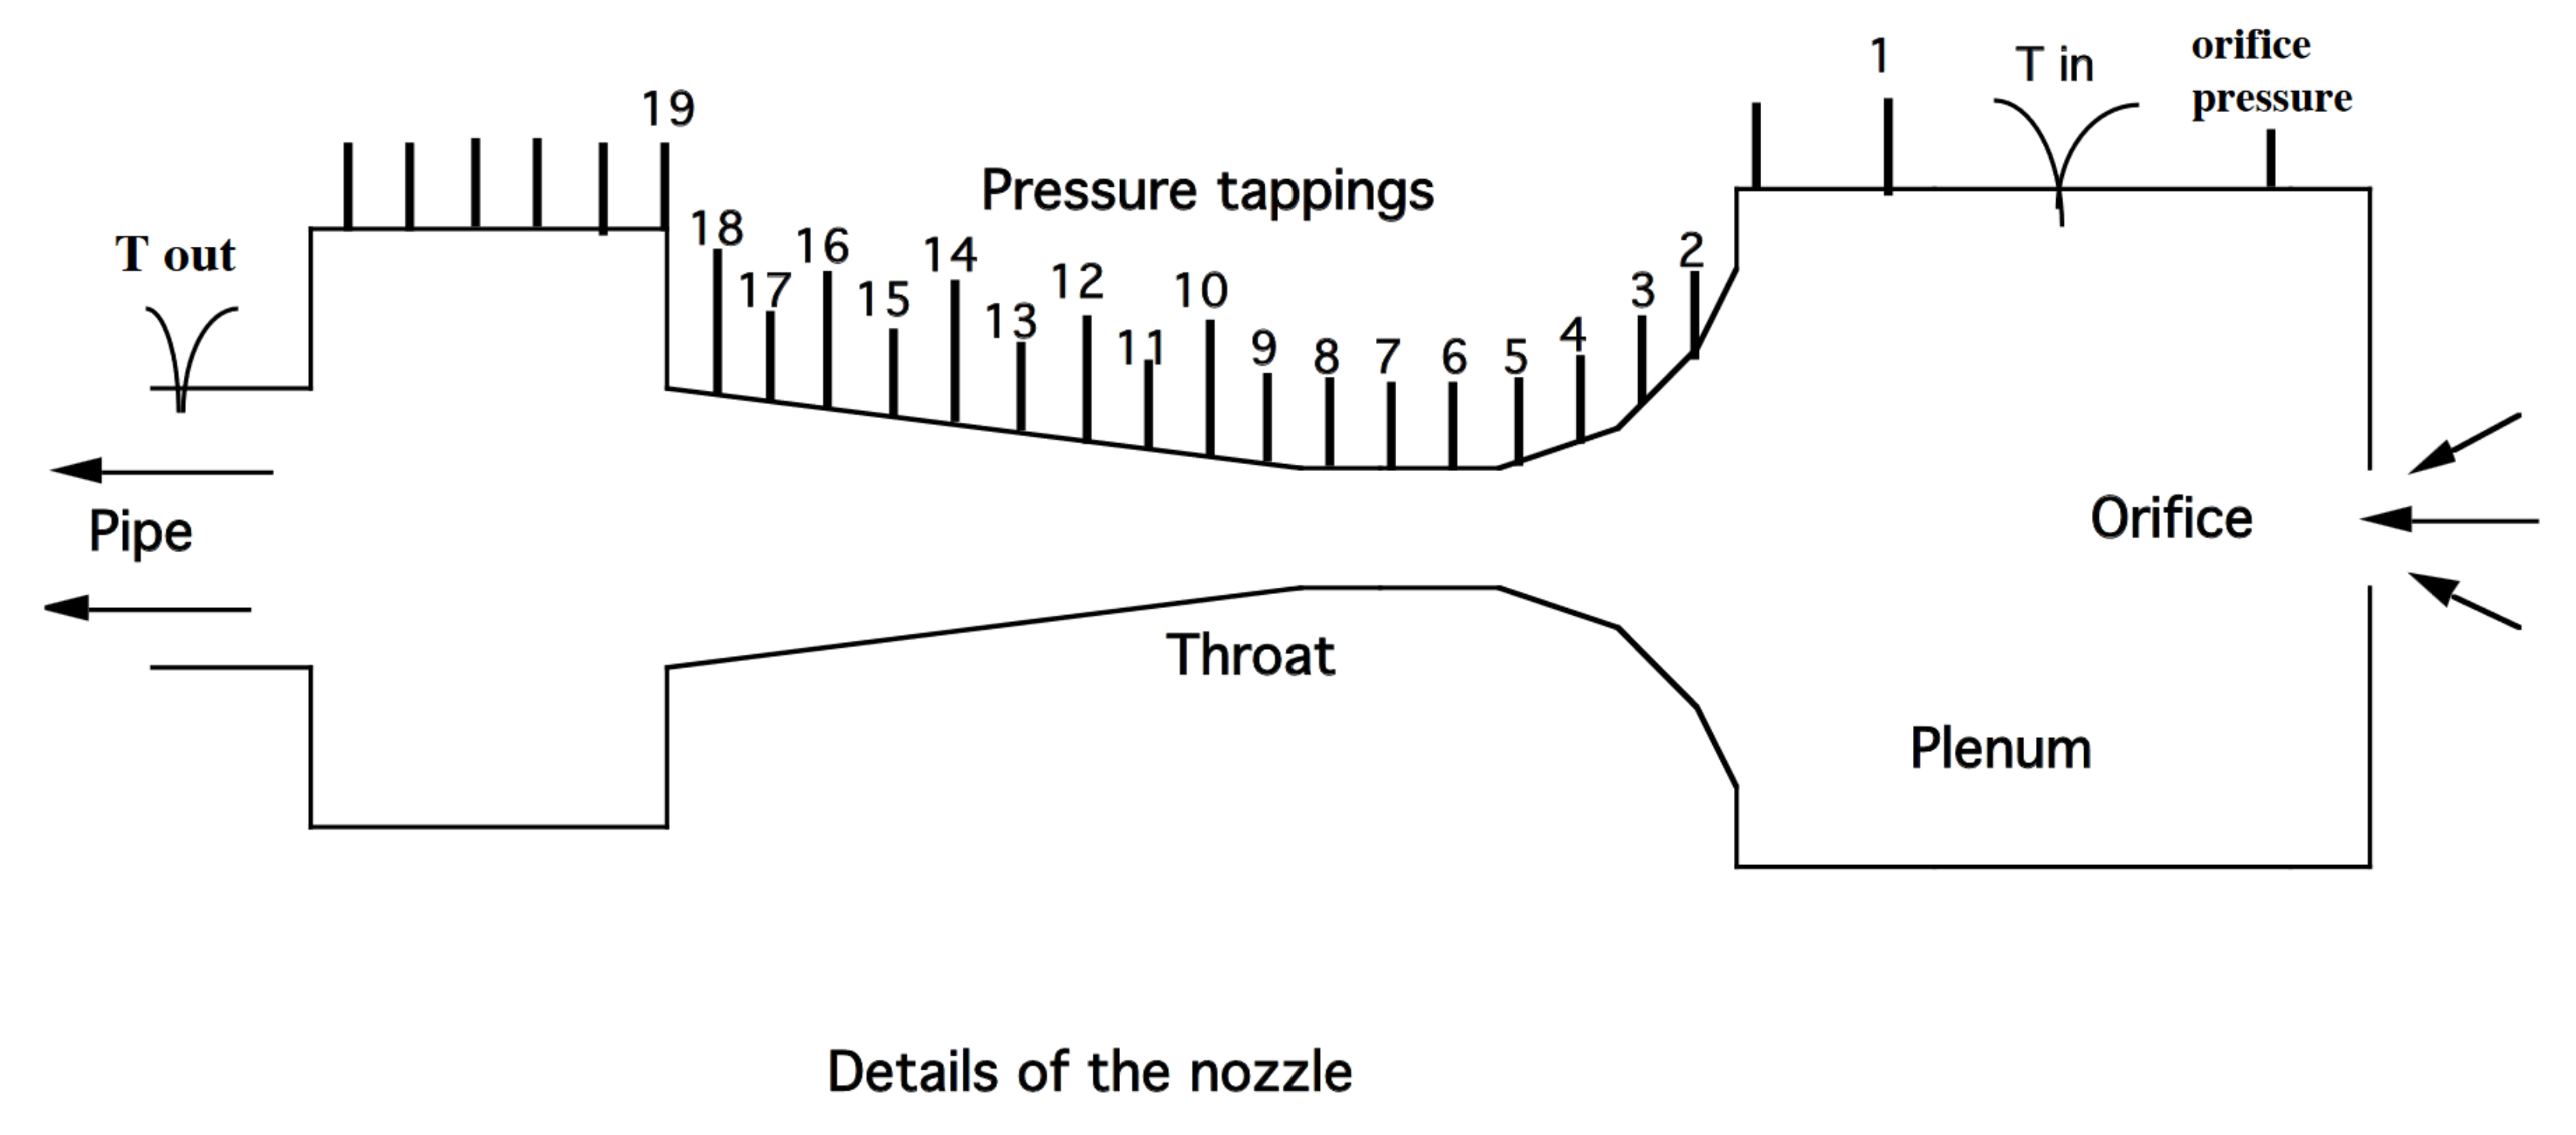
\includegraphics[width=0.8\textwidth]{small_nozzle_layout.png}
    \caption{Layout of Convergent - divergent nozzle}
    \label{fig:figure1}
\end{figure}

Orifice calibration: the diameter of the orifice is 17.47 mm. To a first approximation, assume that
\begin{itemize}
    \item The flow into the orifice is inviscid,
    \item the flow is slow enough to be treated as incompressible with density equal to that in the atmosphere upstream of the orifice (where the velocity is negligible),
    \item the velocity is uniform across the plane of the orifice,
    \item the pressure difference between the orifice plane and the upstream atmosphere is that measured on the
    water manometer
\end{itemize} 

To analyse the validity of the second assumption, consider the case of maximum flow, when the nozzle is choked upstream of the oriface, then its non-dimensional mass flow rate is given by the following equation.
\begin{equation}
    \frac{\dot{m}\sqrt{c_pT_0}}{p_0A^*} = 1.281
\end{equation}
The first assumption is not valid as there is viscous dissipation before the oriface. However, these losses are accounted for by a discharge coefficient $C_d$, which is defined as the ratio of actual discharge to the ideal discharge.
The value of $C_d$ is constant at the high Reynolds numbers considered in this report.
From this, the non-dimensional mass flow rate at the oriface can be calculated using the area ratio of the oriface to the nozzle throat.
The area of the throat is approximately $24\text{mm}^2$, and so the non-dimensional mass flow rate at the oriface is $0.1282$.
At this point, the corresponding density ratio $\rho/\rho_0 = 0.9997 \approx 1$. This means that the density change is negligible and can be ignored.

The third assumption may be valid or not i dont know.

With both the invicid and incompressible assumptions, the ideal flow rate through the orifice can be calculated using the pressure difference between the orifice plane and the upstream atmosphere is that measured on the
water manometer. By applying the Bernoulli equation from the upstream atmosphere (1) to the oriface plane (2),

\begin{equation}
    p_1 = p_2 + \frac{1}{2} \rho_a v_2^2
\end{equation}

Where $A$ and $v_2$ are the cross-sectional area, and velocity at the oriface. The theoretical mass flow rate through the oriface is then given by the following equation.
\begin{equation}
    \dot{m}_{ideal} = \rho_a A v_2 = \rho_a \left( \frac{\pi D^2}{4}\right) \sqrt{\frac{2(p_1-p_2)}{\rho_a}} \;\;\;\;\;\; \text{where} \;\;\;\;\;\ p_2 - p_1 = \rho_w g \Delta h
\end{equation}
Where $\rho_a$ is the density of air and $\rho_w$ is the density of water used for the manometer.
However, the actual flow rate through the orifice differs from the theoretical value as our assumptions are not valid.
This difference is characterised by the discharge coefficient $C_d$ which is defined as the ratio of the actual flow rate to the theoretical flow rate.
\begin{equation}
    \dot{m}_{actual} = C_d \dot{m}_{ideal}
\end{equation}
% https://arc.aiaa.org/doi/pdf/10.2514/6.2019-3651 ?
The discharge coefficient of the oriface is effectively constant over the range of high reynolds numbers considered in this experiment. 

The static pressure at a specific pressure tapping along the nozzle is given by the following equation.
\begin{equation}
    p = p_0 - \rho_{Hg} g \Delta h
\end{equation}
Where $\rho_{Hg}$ is the density of mercury and $\Delta h$ is the height difference of mercury between the specific pressure tapping and atmospheric tapping.
The ratio of this with the stagnation pressure (atmospheric pressure) is the static to stagnation pressure ratio which is plotted below in figure \ref{fig:figure4}.

\begin{figure}[H]
    \centering
    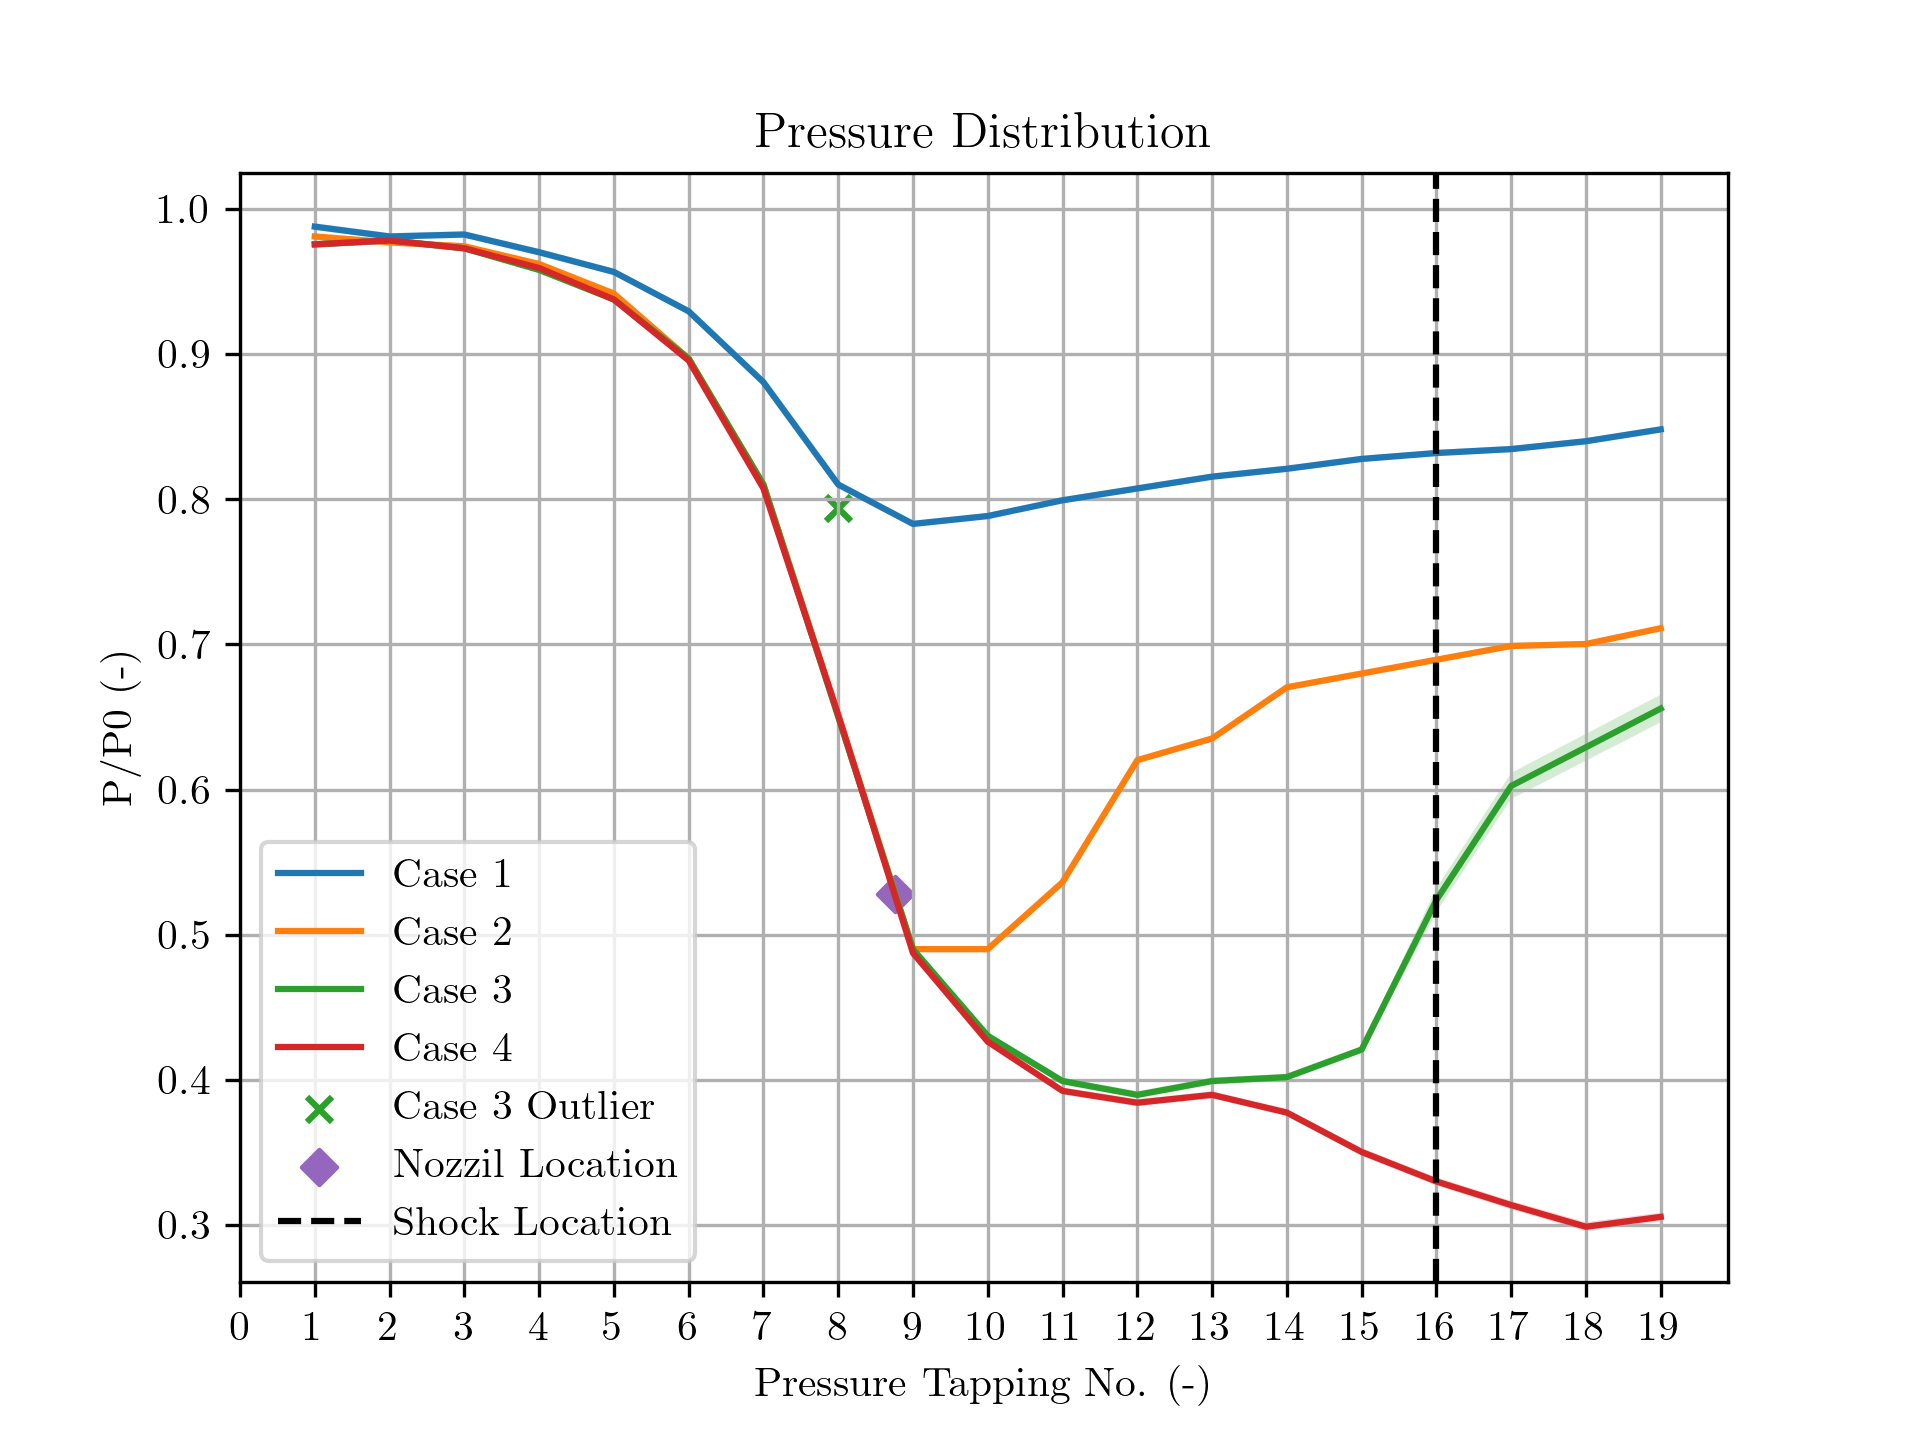
\includegraphics[width=0.8\textwidth]{pressure_ratio_distribution_corrected.png}
    \caption{Static pressure ratio distribution along the nozzle.}
    \label{fig:figure4}
\end{figure}

Figure \ref{fig:figure4} shows the static to stagnant pressure ratio distribution along the nozzle.
Case 2 is when the limiting choke condition is reached, and so for a Mach number of 1.0, the pressure ratio should be 0.5283.
The pressure distribution for Case 2 was then linear interpolated to find the position which was found to be 8.76.

\hfill

Under the assumption that the flow is adiabatic, and isentropic, except for the shock wave in Case 3, (which is accounted for in Equation 8) the Mach number can be calculated from the static pressure ratio as follows:
% M2 = (rp ** - ((g-1)/g) - 1) * 2 / (g - 1)
\begin{equation}
    M = \frac{2}{\gamma - 1} \left[ \left( \frac{p}{p_0} \right) ^ {-\frac{\gamma - 1}{\gamma}} - 1 \right]
\end{equation}
This is plotted in figure \ref{fig:figure5} below.

\begin{figure}[H]
    \centering
    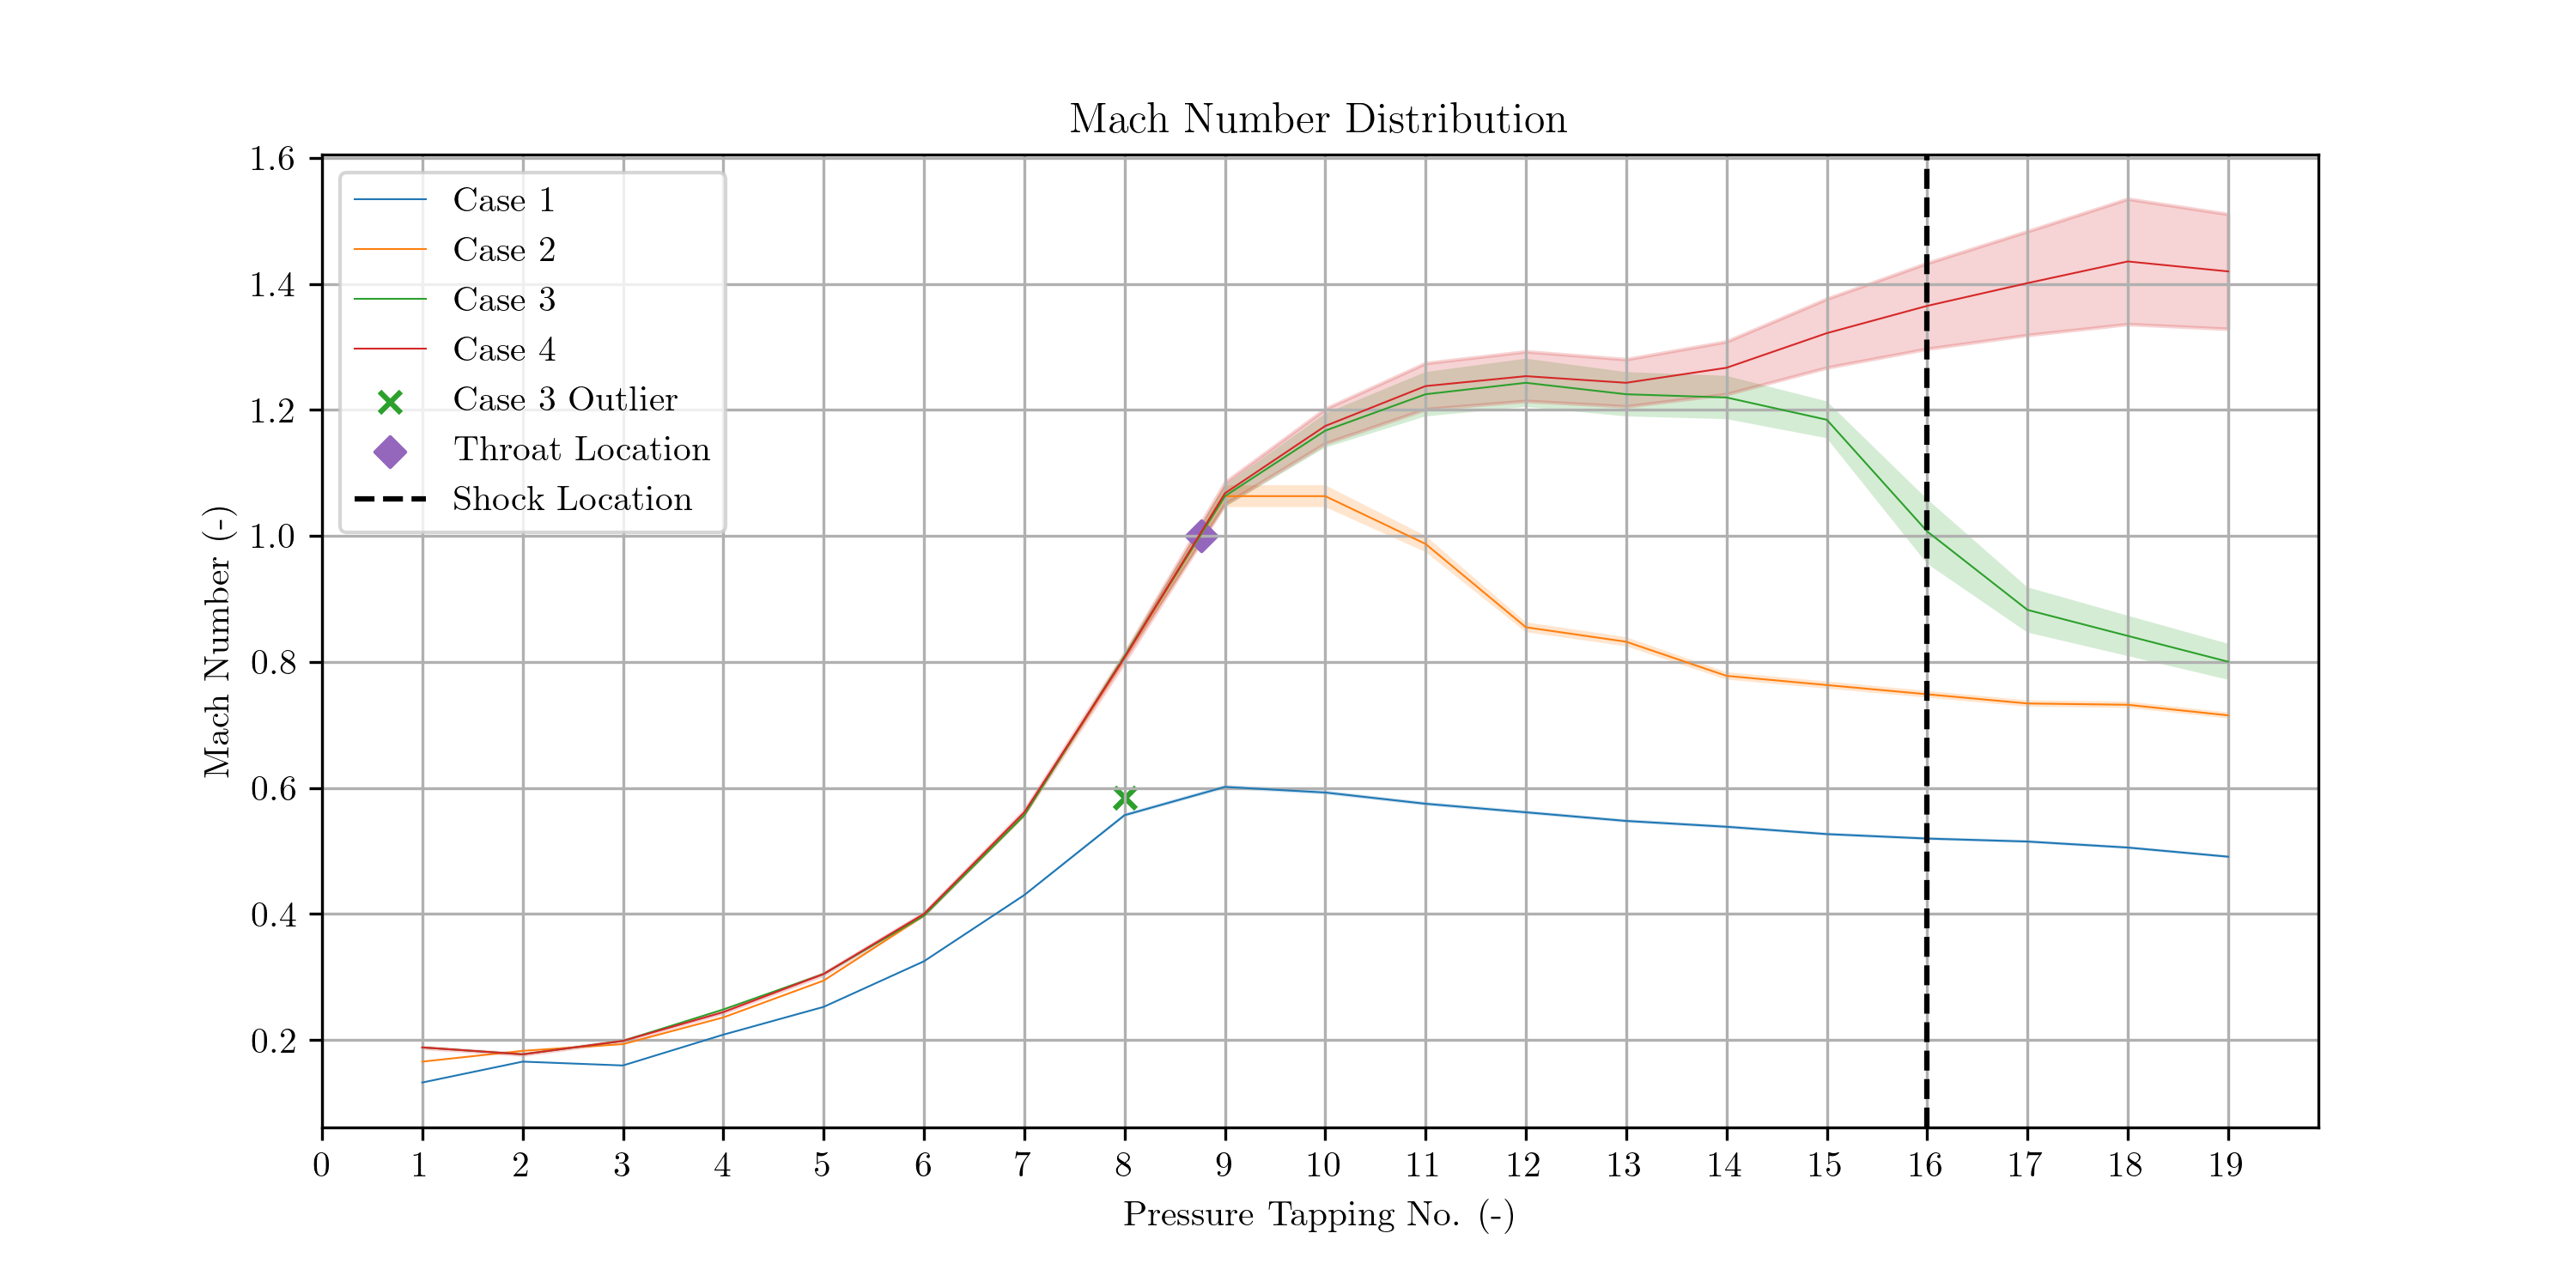
\includegraphics[width=0.8\textwidth]{mach_number_distribution_corrected.png}
    \caption{Figure 1}
    \label{fig:figure5}
\end{figure}
The plot of Mach number against position along the nozzle is shown below in figure \ref{fig:figure5}.

\begin{center}
    \captionof{table}{Exit and throat Mach numbers for each case.}
    \begin{tabular}{|c|c|c|c|}
    \hline 
    Case & Throat Mach No.  & Exit Mach No. & Mass flow rate\\
     & (-) & (-) & kg/s \\
    \hline 
    1 & $0.602$ & $0.491$ & $ 4.25 \times 10^{-3} $ \\
    2 & $1.063$ & $0.715$ & $ 4.96 \times 10^{-3} $ \\
    3 & $1.063$ & - & $ 4.96 \times 10^{-3} $ \\
    4 & $1.068$ & $1.420$ & $ 4.96 \times 10^{-3} $ \\
    \hline
    \end{tabular}
    \label{tab:1}
\end{center}

From looking at Case 3 where the shock wave is to be expected in the nozzle divergence, the Mach number increases from the throat to the exit of the nozzle then gradually decreases again.
The lack of sharp jump in pressure is mainly due to the fact that the measurements taken at the wall are smeared by the interaction between the boundary layer and the shock wave.
The shock position is estimated to be at position 16.
% As a rough guess the shock in the core of the nozzle is assumed to be situated approximately at the axial position where $p/p_{0s}$ takes a value equal to $p/p_0$ for $M = 1$.
% what does this mean

The Mach number after the shock can be calculated from the Mach number before the shock. This value is taken from position 16 of Case 4 to avoid shock boundary layer effects.
% Ms from M
\begin{equation}
    M_s = \left( \frac{1 + \frac{\gamma - 1}{2} M^2}{\gamma M^2 - \frac{\gamma - 1}{2}} \right) ^ \frac{1}{2}
\end{equation}

Then the ratio of stagnant pressure ratios before and after the shock as a function of the Mach number before the shock is given by the following equation:
\begin{equation}
    \frac{p_{0s}}{p} = \left( \frac{\gamma + 1}{2} M^2 \right) ^ \frac{\gamma}{\gamma - 1} \left( \frac{2\gamma}{\gamma+1}M^2 - \frac{\gamma-1}{\gamma+1}\right) ^ \frac{1}{1 - \gamma}
\end{equation}
And so at position 16, before the shock $M = 1.365$ the stagnant pressure ratio is $p_{0s}/p = 0.9665$.
In figure \ref{fig:figure4} the static to stagnation pressure ratio of case 3, after the shock is divided by this value to give the correct static pressure ratio after the shock.
Figure \ref{fig:figure5} uses the corrected pressure ratios to calculate the Mach number after the shock using the same equation 5.


\begin{figure}[H]
    \centering
    \begin{subfigure}[t]{0.48\textwidth}
        \centering
        \includegraphics[width=1\textwidth]{shadowgraph_annotations/slide1.PNG}
        \caption{Shock wave in working section before sensors}

        \label{fig:figure6}
    \end{subfigure}
    ~
    \begin{subfigure}[t]{0.48\textwidth}
        \centering
        \includegraphics[width=1\textwidth]{shadowgraph_annotations/slide2.PNG}
        \caption{Working state and bow shock of pitot probe}
        \label{fig:figure7}
    \end{subfigure}
    \caption{Shadowgraph images of the supersonic wind tunnel}
\end{figure}

Figure \ref{fig:figure6} shows the shock wave in the working section of the supersonic wind tunnel before the pressure sensors.
Shock waves of high density gradient are visible in the image from dark regions of the shadowgraph, where darker regions indicate stronger shock waves.
At the boundary layers at the top and bottom of the tunnel, the flow appears to travel through two shockwaves.
After the first shockwave the flow near the boundary layer is subsonic, but then must be accelerated again to supersonic speeds before the second, weaker shock.


\begin{figure}[H]
    \centering
    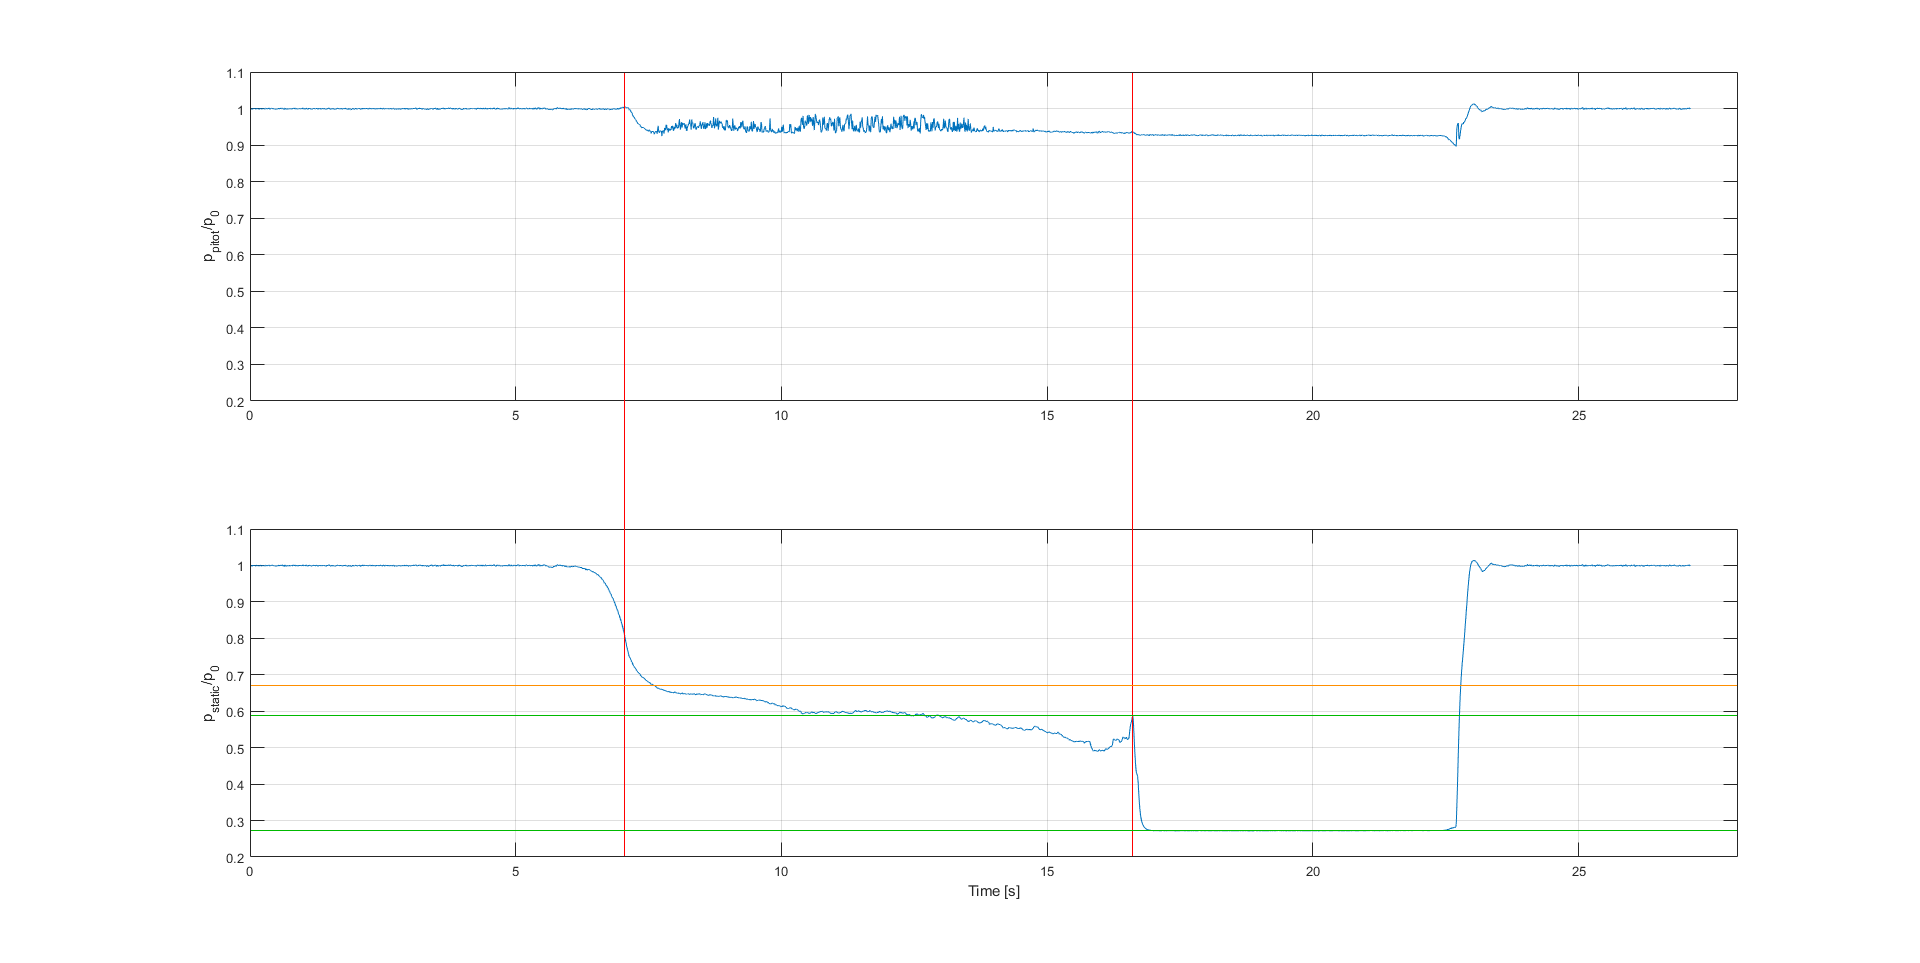
\includegraphics[width=1\textwidth]{tunnel_pressures_annotated.png}
    \caption{Annotated readings of the pressure sensors over time during the experiment. Top graph shows the stagnation pressure ratio, and the bottom graph shows the static pressure ratio.}
    \label{fig:figure8}
\end{figure}

Figure \ref{fig:figure8} shows the annotated readings of the pressure sensors over time during the experiment.
The green and red dots indicates the time at which the tunnel was switched on and off respectively.
It can be observed that before the first vertical red line, the static pressure decreases which corresponds to the subsonic flow accelerating.
At the first red line the stagnation pressure falls as the normal shock wave is formed upstream of the sensors by the, now supersonic, flow downstream of the throat.
The stagnation pressure readings then becomes very noisy as the shock wave moves further downstream due to complex shock boundary layer interactions.
The static pressure ratio slowly decreases over the next several seconds, indicating an acceleration in the flow, before quickly increasing again.
This may be due to the boundary layer growing and then shrinking rapidly, acting similarly to a convergent divergent nozzle, as the shock wave moves closer to the sensors.
The second vertical red line shows where the shock wave passes the sensors and static pressure drops significantly.

After the shock has passed, the bottom green line shows a static pressure ratio of around $p/p_0 = 0.275$. This corresponds to a Mach number of 1.49, which is very close to the set operating point of Mach 1.5.
From the databook, at Mach 1.5 the pressure ratio accross the shock should be $p_s/p = 2.4583$.
Multiplying this by the measured static pressure ratio after the shock passes, gives us the theoetical static pressure ratio before the shock passed, which is $p_s/p_0 = 0.275 \times 2.4583 = 0.676$, and is shown by the orange horizontal line.
The actual pressure ratio behind the shock, given by the pressure at the time before the shock passes the sensors, is shown by the top green line at $p_s/p_0 = 0.59$.
This shows that the actual pressure drop accross the shock is less than the theoretical value for Mach 1.5.
It seems that the strength of the shock wave is reduced, and the flow after the shock is at a higher Mach number than expected due to the boundary layer effects.

The pitot probe should show an increase in stagnation pressure after the shock wave passes, however it can be observed that this remains nearly unchanged.
However, it can be observed from figure \ref{fig:figure7} that a bow shock forms in front of the pitot probe and so the shock effectively never passes the probe.

\end{document}
